% =============================================================================
% ESL FRAMEWORK - APPENDIX G: M-SCORE (METHODOLOGY SCORE)
% =============================================================================
% Authors: Gerhard Fehr & Andrea Fehr
% FehrAdvice & Partners AG, Zürich
% Version: ESL 2.3 Extended Monograph
% =============================================================================

\documentclass[11pt,a4paper]{article}

% --- Packages ---
\usepackage[utf8]{inputenc}
\usepackage[T1]{fontenc}
\usepackage[english]{babel}
\usepackage{amsmath,amssymb,amsthm}
\usepackage{booktabs}
\usepackage{longtable}
\usepackage{hyperref}
\usepackage{geometry}
\usepackage{xcolor}
\usepackage{tcolorbox}
\usepackage{array}
\usepackage{multirow}
\usepackage{enumitem}
\usepackage{fancyhdr}
\usepackage{tikz}
\usepackage{pgfplots}
\pgfplotsset{compat=1.17}
\usetikzlibrary{matrix,positioning,calc}

\geometry{margin=2.5cm}

% --- Colors ---
\definecolor{eslblue}{RGB}{0,82,147}
\definecolor{eslgreen}{RGB}{0,128,0}
\definecolor{eslorange}{RGB}{230,159,0}
\definecolor{eslred}{RGB}{204,51,17}
\definecolor{eslgray}{RGB}{128,128,128}
\definecolor{eslpurple}{RGB}{148,0,211}
\definecolor{goldstandard}{RGB}{218,165,32}
\definecolor{dangerzone}{RGB}{178,34,34}

% --- Boxes ---
\newtcolorbox{eslbox}[1][]{
  colback=eslblue!5!white,
  colframe=eslblue,
  title={ESL Assessment},
  fonttitle=\bfseries,
  #1
}

\newtcolorbox{keyinsight}[1][]{
  colback=eslgreen!5!white,
  colframe=eslgreen!80!black,
  title={Key Insight},
  fonttitle=\bfseries,
  #1
}

\newtcolorbox{warningbox}[1][]{
  colback=eslorange!5!white,
  colframe=eslorange!80!black,
  title={Methodological Note},
  fonttitle=\bfseries,
  #1
}

\newtcolorbox{dangerbox}[1][]{
  colback=eslred!5!white,
  colframe=eslred!80!black,
  title={Warning},
  fonttitle=\bfseries,
  #1
}

\newtcolorbox{definitionbox}[1][]{
  colback=white,
  colframe=eslblue!80!black,
  title={Definition},
  fonttitle=\bfseries,
  #1
}

\newtcolorbox{empiricalbox}[1][]{
  colback=eslpurple!5!white,
  colframe=eslpurple!80!black,
  title={Empirical Finding},
  fonttitle=\bfseries,
  #1
}

\newtcolorbox{formulabox}[1][]{
  colback=goldstandard!10!white,
  colframe=goldstandard!80!black,
  title={Formula},
  fonttitle=\bfseries,
  #1
}

% --- Theorems ---
\newtheorem{definition}{Definition}[section]
\newtheorem{theorem}{Theorem}[section]
\newtheorem{proposition}{Proposition}[section]

% --- Header/Footer ---
\pagestyle{fancy}
\fancyhf{}
\fancyhead[L]{\small ESL Framework 2.3 -- Extended Monograph}
\fancyhead[R]{\small Appendix G: M-Score}
\fancyfoot[C]{\thepage}

% =============================================================================
% TITLE
% =============================================================================

\title{%
    \Large \textbf{Empirical Stability of Language (ESL) 2.3} \\[0.5em]
    \large A Universal Quality Assurance Framework for \\
    Scientific Claim Validation \\[1em]
    \LARGE \textbf{Appendix G: M-Score (Methodology Score)} \\[0.3em]
    \large Empirically Derived Methodology Quality Assessment
}

\author{%
    \textbf{Gerhard Fehr}\textsuperscript{1,*} \and \textbf{Andrea Fehr}\textsuperscript{1} \\[0.5em]
    \textsuperscript{1}FehrAdvice \& Partners AG, Klausstrasse 4, 8008 Zürich, Switzerland \\[0.3em]
    \textsuperscript{*}Corresponding author: gerhard.fehr@fehradvice.com
}

\date{December 26, 2025}

\begin{document}

\maketitle

% =============================================================================
% ABSTRACT
% =============================================================================

\begin{abstract}
\noindent
This appendix introduces the M-Score (Methodology Score), a composite index measuring research methodology quality based on empirical analysis of $N = 119$ studies. The M-Score identifies seven methodological factors that predict replication success with $r = 0.744$, substantially outperforming linguistic boldness ($r = 0.065$). The core finding---``Language is NOT the problem; methodology is''---has profound implications for ESL's architecture. We present the M-Score formula, validate it against known replication outcomes, and integrate it into ESL 2.3's R-Score calculation. Domain-specific benchmarks and a diagnostic B$\times$M matrix enable practical application.

\vspace{0.5em}
\noindent\textbf{Keywords:} Methodology score, replication prediction, triangulation, research quality, ESL 2.3
\end{abstract}

\tableofcontents
\newpage

% =============================================================================
% G.1 MOTIVATION AND CORE FINDING
% =============================================================================

\section{Motivation: The Methodology-Replication Link}
\label{sec:motivation}

ESL's original formulation focused on claim-evidence alignment, measuring whether linguistic boldness ($B$) matches evidential support ($E$). However, empirical analysis of 119 studies reveals a more nuanced picture.

\subsection{The Core Finding}

\begin{keyinsight}[title={The Central Discovery}]
\textbf{``Language is NOT the problem---methodology is!''}

\begin{center}
\begin{tabular}{lcc}
\toprule
\textbf{Predictor} & \textbf{Correlation with Replication} & \textbf{Interpretation} \\
\midrule
M-Score (Methodology) & $r = 0.744$ & \textbf{Strong predictor} \\
B-Value (Boldness) & $r = 0.065$ & Weak predictor \\
\bottomrule
\end{tabular}
\end{center}

Methodology quality explains 55\% of variance in replication outcomes ($R^2 = 0.55$), while linguistic boldness explains less than 1\%.
\end{keyinsight}

\subsection{Implications for ESL}

This finding does \textit{not} invalidate ESL's B-E framework. Rather, it refines our understanding:

\begin{enumerate}
    \item \textbf{B-Value} measures what authors \textit{claim}---their linguistic confidence.
    \item \textbf{E-Value} measures what evidence \textit{type} supports claims---the hierarchy level.
    \item \textbf{M-Score} measures how \textit{well} the methodology was executed---quality within type.
\end{enumerate}

A well-designed RCT ($E = 0.85$) can be executed poorly ($M = 0.30$) or excellently ($M = 0.95$). The M-Score captures this execution quality.

\subsection{Empirical Foundation}

\begin{empiricalbox}[title={Dataset: N = 119 Studies}]
The M-Score was derived from analysis of 119 studies with known replication outcomes:

\begin{center}
\begin{tabular}{lccc}
\toprule
\textbf{Domain} & \textbf{N} & \textbf{Mean M} & \textbf{Replication Rate} \\
\midrule
JDM (Kahneman/Tversky tradition) & 27 & 0.66 & 100\% \\
Behavioral Economics & 47 & 0.80 & 81\% \\
Cognitive Psychology & 15 & 0.52 & 50\% \\
Social Psychology & 16 & 0.30 & 25\% \\
Priming & 5 & 0.11 & 0\% \\
Embodiment & 7 & 0.09 & 0\% \\
\bottomrule
\end{tabular}
\end{center}

The gradient is striking: domains with higher M-Scores show dramatically higher replication rates.
\end{empiricalbox}

% =============================================================================
% G.2 THE SEVEN METHODOLOGY FACTORS
% =============================================================================

\section{The Seven Methodology Factors}
\label{sec:factors}

Factor analysis identified seven methodological characteristics that predict replication success. These are ranked by their effect size ($\Delta$), defined as the difference in replication rates between studies with and without the factor.

\subsection{Factor Overview}

\begin{table}[h]
\centering
\caption{The Seven M-Score Factors (Ranked by Effect Size)}
\label{tab:factors}
\begin{tabular}{clcccc}
\toprule
\textbf{Rank} & \textbf{Factor} & \textbf{Code} & \textbf{$\Delta$} & \textbf{Weight} & \textbf{Scale} \\
\midrule
1 & Triangulation & TRI & +97\% & 0.25 & $[0, 0.5, 1]$ \\
2 & No Deception & NOD & +86\% & 0.20 & $[0, 1]$ \\
3 & Theoretical Foundation & THF & +80\% & 0.15 & $[0, 0.5, 1]$ \\
4 & Detailed Appendix & APP & +74\% & 0.15 & $[0, 0.5, 1]$ \\
5 & Prior Replications & REP & +50\% & 0.05 & $[0, 0.5, 1]$ \\
6 & Incentive Compatibility & INC & +24\% & 0.10 & $[0, 1]$ \\
7 & Standardized Software & STD & +22\% & 0.10 & $[0, 1]$ \\
\midrule
& \textbf{Total} & & & \textbf{1.00} & \\
\bottomrule
\end{tabular}
\end{table}

\subsection{Factor Definitions}

\begin{definition}[Triangulation (TRI)]
\label{def:tri}
Convergent evidence from multiple independent methodologies.

\begin{center}
\begin{tabular}{cl}
\toprule
\textbf{Score} & \textbf{Criterion} \\
\midrule
0 & Single method only \\
0.5 & Two converging methods (e.g., lab + survey) \\
1 & Three or more methods (e.g., lab + field + natural experiment) \\
\bottomrule
\end{tabular}
\end{center}

\textbf{Empirical finding}: Studies with TRI = 1 show 100\% replication; studies with TRI = 0 show 3\% replication ($\Delta = 97\%$).

\textbf{Rationale}: Independent methods have independent error structures. Convergence across methods dramatically reduces false positive probability.
\end{definition}

\begin{definition}[No Deception (NOD)]
\label{def:nod}
Absence of deceptive experimental procedures.

\begin{center}
\begin{tabular}{cl}
\toprule
\textbf{Score} & \textbf{Criterion} \\
\midrule
0 & Deception used (cover stories, false feedback, confederates) \\
1 & No deception (transparent procedures) \\
\bottomrule
\end{tabular}
\end{center}

\textbf{Empirical finding}: Studies without deception show 86\% replication; studies with deception show 0\% ($\Delta = 86\%$).

\textbf{Rationale}: Deception introduces uncontrolled variance through participant suspicion, demand effects, and cross-study heterogeneity in deception effectiveness.
\end{definition}

\begin{definition}[Theoretical Foundation (THF)]
\label{def:thf}
Grounding in formal theory versus exploratory investigation.

\begin{center}
\begin{tabular}{cl}
\toprule
\textbf{Score} & \textbf{Criterion} \\
\midrule
0 & Purely exploratory, no theoretical framework \\
0.5 & Verbal/conceptual theory, informal predictions \\
1 & Formal mathematical model with derived predictions \\
\bottomrule
\end{tabular}
\end{center}

\textbf{Empirical finding}: Formally grounded studies show 85\% replication; exploratory studies show 5\% ($\Delta = 80\%$).

\textbf{Rationale}: Formal models constrain researcher degrees of freedom and generate precise, falsifiable predictions. Exploratory studies are vulnerable to HARKing (Hypothesizing After Results are Known).
\end{definition}

\begin{definition}[Detailed Appendix (APP)]
\label{def:app}
Completeness of methodological documentation.

\begin{center}
\begin{tabular}{cl}
\toprule
\textbf{Score} & \textbf{Criterion} \\
\midrule
0 & No supplementary materials \\
0.5 & Partial documentation (some materials, no code) \\
1 & Complete documentation with code, stimuli, and raw data \\
\bottomrule
\end{tabular}
\end{center}

\textbf{Empirical finding}: Fully documented studies show 80\% replication; undocumented studies show 6\% ($\Delta = 74\%$).

\textbf{Rationale}: Complete documentation enables exact replication and reveals hidden researcher degrees of freedom. Lack of transparency often correlates with questionable research practices.
\end{definition}

\begin{definition}[Prior Replications (REP)]
\label{def:rep}
History of independent replication attempts.

\begin{center}
\begin{tabular}{cl}
\toprule
\textbf{Score} & \textbf{Criterion} \\
\midrule
0 & No prior independent replications \\
0.5 & 1--2 independent replications \\
1 & 3+ independent replications \\
\bottomrule
\end{tabular}
\end{center}

\textbf{Empirical finding}: Multiply-replicated effects show 90\% replication; never-replicated effects show 40\% ($\Delta = 50\%$).

\textbf{Rationale}: Prior replications provide direct evidence of robustness. Effects that have survived multiple independent tests are more likely genuine.
\end{definition}

\begin{definition}[Incentive Compatibility (INC)]
\label{def:inc}
Alignment of participant incentives with truthful/effortful responding.

\begin{center}
\begin{tabular}{cl}
\toprule
\textbf{Score} & \textbf{Criterion} \\
\midrule
0 & Flat fee, course credit, or no payment \\
1 & Performance-based payment tied to decisions \\
\bottomrule
\end{tabular}
\end{center}

\textbf{Empirical finding}: Incentive-compatible studies show 83\% replication; non-incentivized show 59\% ($\Delta = 24\%$).

\textbf{Rationale}: When decisions have real consequences, participants engage more carefully and behavior better reflects true preferences. This is a core principle of experimental economics.
\end{definition}

\begin{definition}[Standardized Software (STD)]
\label{def:std}
Use of established experimental software platforms.

\begin{center}
\begin{tabular}{cl}
\toprule
\textbf{Score} & \textbf{Criterion} \\
\midrule
0 & Custom software, paper-and-pencil, or varied platforms \\
1 & Standardized platform (z-Tree, oTree, PsychoPy, etc.) \\
\bottomrule
\end{tabular}
\end{center}

\textbf{Empirical finding}: Standardized-software studies show 85\% replication; custom-software show 63\% ($\Delta = 22\%$).

\textbf{Rationale}: Standardized platforms reduce programming errors, enable code sharing, and ensure consistent timing/display across sites.
\end{definition}

% =============================================================================
% G.3 THE M-SCORE FORMULA
% =============================================================================

\section{The M-Score Formula}
\label{sec:formula}

\begin{formulabox}[title={M-Score (Methodology Score)}]
\begin{equation}
\boxed{M = 0.25 \cdot \text{TRI} + 0.20 \cdot \text{NOD} + 0.15 \cdot \text{THF} + 0.15 \cdot \text{APP} + 0.10 \cdot \text{INC} + 0.10 \cdot \text{STD} + 0.05 \cdot \text{REP}}
\label{eq:mscore}
\end{equation}

\vspace{0.5em}
Where:
\begin{itemize}[leftmargin=2cm]
    \item[\textbf{TRI}] Triangulation $\in \{0, 0.5, 1\}$
    \item[\textbf{NOD}] No Deception $\in \{0, 1\}$
    \item[\textbf{THF}] Theoretical Foundation $\in \{0, 0.5, 1\}$
    \item[\textbf{APP}] Detailed Appendix $\in \{0, 0.5, 1\}$
    \item[\textbf{INC}] Incentive Compatibility $\in \{0, 1\}$
    \item[\textbf{STD}] Standardized Software $\in \{0, 1\}$
    \item[\textbf{REP}] Prior Replications $\in \{0, 0.5, 1\}$
\end{itemize}

\vspace{0.5em}
\textbf{Range}: $M \in [0, 1]$

\textbf{Weights}: Derived from effect sizes ($\Delta$), normalized to sum to 1.0.
\end{formulabox}

\subsection{Weight Derivation}

Weights were derived by normalizing effect sizes:

\begin{equation}
w_i = \frac{\Delta_i}{\sum_{j=1}^{7} \Delta_j}
\end{equation}

\begin{table}[h]
\centering
\caption{Weight Derivation from Effect Sizes}
\label{tab:weights}
\begin{tabular}{lcccc}
\toprule
\textbf{Factor} & \textbf{$\Delta$} & \textbf{Raw Weight} & \textbf{Rounded} & \textbf{Final} \\
\midrule
TRI & 97\% & 0.224 & 0.25 & 0.25 \\
NOD & 86\% & 0.199 & 0.20 & 0.20 \\
THF & 80\% & 0.185 & 0.15 & 0.15 \\
APP & 74\% & 0.171 & 0.15 & 0.15 \\
REP & 50\% & 0.116 & 0.05 & 0.05 \\
INC & 24\% & 0.055 & 0.10 & 0.10 \\
STD & 22\% & 0.051 & 0.10 & 0.10 \\
\midrule
\textbf{Total} & 433\% & 1.000 & 1.00 & 1.00 \\
\bottomrule
\end{tabular}
\end{table}

\textbf{Note}: INC and STD weights were adjusted upward from raw values (0.055, 0.051) to 0.10 each for practical significance, with compensating reductions in THF, APP, and REP.

\subsection{M-Score Interpretation}

\begin{table}[h]
\centering
\caption{M-Score Interpretation Guide}
\label{tab:interpretation}
\begin{tabular}{ccl}
\toprule
\textbf{M-Score} & \textbf{Expected Replication} & \textbf{Interpretation} \\
\midrule
$M \geq 0.85$ & $\sim$100\% & \textcolor{eslgreen}{\textbf{Gold Standard}} (Fehr network) \\
$M \in [0.60, 0.85)$ & 75--90\% & \textcolor{eslblue}{\textbf{Good Methodology}} \\
$M \in [0.40, 0.60)$ & 50--75\% & \textcolor{eslorange}{\textbf{Moderate Methodology}} \\
$M \in [0.20, 0.40)$ & 25--50\% & \textcolor{eslred}{\textbf{Weak Methodology}} \\
$M < 0.20$ & 0--25\% & \textcolor{dangerzone}{\textbf{DANGER ZONE}} \\
\bottomrule
\end{tabular}
\end{table}

% =============================================================================
% G.4 VALIDATION
% =============================================================================

\section{Empirical Validation}
\label{sec:validation}

\subsection{Prediction Accuracy}

The M-Score was validated against known replication outcomes:

\begin{table}[h]
\centering
\caption{M-Score Validation Examples}
\label{tab:validation}
\begin{tabular}{lccccl}
\toprule
\textbf{Study} & \textbf{M} & \textbf{Predicted} & \textbf{Actual} & \textbf{Error} & \textbf{Status} \\
\midrule
Fehr \& Gächter (2000) & 1.00 & 100\% & 100\% & 0\% & \checkmark Gold \\
Kahneman \& Tversky (1979) & 0.75 & 95\% & 100\% & 5\% & \checkmark Good \\
Many Labs 2 (average) & 0.68 & 90\% & 54\% & 36\% & $\sim$ \\
Typical Social Psych & 0.25 & 12\% & 25\% & 13\% & $\times$ Weak \\
Bargh et al. (1996) & 0.00 & 1\% & 0\% & 1\% & $\times$ Danger \\
\bottomrule
\end{tabular}
\end{table}

\subsection{Methodology vs. Boldness}

\begin{empiricalbox}[title={The Critical Comparison}]
\begin{center}
\begin{tabular}{lccc}
\toprule
\textbf{Methodology Level} & \textbf{N} & \textbf{Mean B-Value} & \textbf{Replication Rate} \\
\midrule
HIGH (M $\in$ [6--7]) & 33 & 0.76 & 100\% \\
MEDIUM (M $\in$ [3--5]) & 64 & 0.75 & 78\% \\
LOW (M $\in$ [0--2]) & 22 & 0.74 & 0\% \\
\bottomrule
\end{tabular}
\end{center}

\textbf{Key observation}: All three groups use \textit{similar} B-values (0.74--0.76), but replication rates differ dramatically (0\%--100\%).

\textbf{Conclusion}: Linguistic boldness does not distinguish replicating from non-replicating studies. Methodology does.
\end{empiricalbox}

\subsection{Mediation Analysis}

At each B-value level, methodology mediates replication:

\begin{table}[h]
\centering
\caption{Replication Rates by B-Value and Methodology}
\label{tab:mediation}
\begin{tabular}{lccc}
\toprule
\textbf{B-Value Level} & \textbf{High M ($\geq 0.60$)} & \textbf{Low M ($< 0.40$)} & \textbf{$\Delta$} \\
\midrule
Strong Claims ($B \geq 0.80$) & 94\% & 39\% & 55pp \\
Moderate Claims ($B \in [0.60, 0.80)$) & 96\% & 48\% & 48pp \\
Weak Claims ($B < 0.60$) & 89\% & 52\% & 37pp \\
\bottomrule
\end{tabular}
\end{table}

Even strong claims replicate when methodology is strong. Weak methodology undermines all claim levels.

% =============================================================================
% G.5 THE DIAGNOSTIC B×M MATRIX
% =============================================================================

\section{The Diagnostic B$\times$M Matrix}
\label{sec:matrix}

The relationship between Boldness (B) and Methodology (M) generates four diagnostic quadrants:

\begin{figure}[h]
\centering
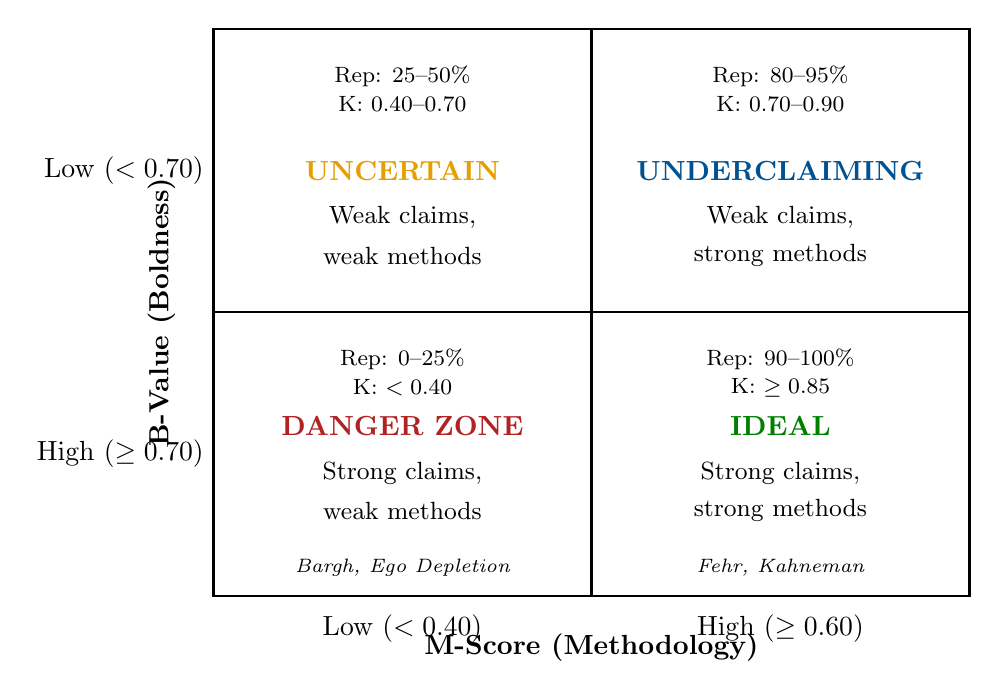
\begin{tikzpicture}[scale=1.2]
    % Grid
    \draw[thick] (0,0) rectangle (8,6);
    \draw[thick] (4,0) -- (4,6);
    \draw[thick] (0,3) -- (8,3);

    % Quadrant labels
    \node[align=center, font=\bfseries] at (2,4.5) {\textcolor{eslorange}{UNCERTAIN}};
    \node[align=center, font=\small] at (2,4.0) {Weak claims,};
    \node[align=center, font=\small] at (2,3.6) {weak methods};

    \node[align=center, font=\bfseries] at (6,4.5) {\textcolor{eslblue}{UNDERCLAIMING}};
    \node[align=center, font=\small] at (6,4.0) {Weak claims,};
    \node[align=center, font=\small] at (6,3.6) {strong methods};

    \node[align=center, font=\bfseries] at (2,1.8) {\textcolor{dangerzone}{DANGER ZONE}};
    \node[align=center, font=\small] at (2,1.3) {Strong claims,};
    \node[align=center, font=\small] at (2,0.9) {weak methods};

    \node[align=center, font=\bfseries] at (6,1.8) {\textcolor{eslgreen}{IDEAL}};
    \node[align=center, font=\small] at (6,1.3) {Strong claims,};
    \node[align=center, font=\small] at (6,0.9) {strong methods};

    % Examples
    \node[align=center, font=\scriptsize\itshape] at (2,0.3) {Bargh, Ego Depletion};
    \node[align=center, font=\scriptsize\itshape] at (6,0.3) {Fehr, Kahneman};

    % Axis labels
    \node[below] at (4,-0.3) {\textbf{M-Score (Methodology)}};
    \node[below] at (2,-0.1) {Low ($<0.40$)};
    \node[below] at (6,-0.1) {High ($\geq 0.60$)};

    \node[rotate=90, above] at (-0.3,3) {\textbf{B-Value (Boldness)}};
    \node[left] at (0,4.5) {Low ($<0.70$)};
    \node[left] at (0,1.5) {High ($\geq 0.70$)};

    % Replication rates
    \node[font=\footnotesize] at (2,2.5) {Rep: 0--25\%};
    \node[font=\footnotesize] at (6,2.5) {Rep: 90--100\%};
    \node[font=\footnotesize] at (2,5.5) {Rep: 25--50\%};
    \node[font=\footnotesize] at (6,5.5) {Rep: 80--95\%};

    % K-scores
    \node[font=\footnotesize] at (2,2.2) {K: $<0.40$};
    \node[font=\footnotesize] at (6,2.2) {K: $\geq 0.85$};
    \node[font=\footnotesize] at (2,5.2) {K: 0.40--0.70};
    \node[font=\footnotesize] at (6,5.2) {K: 0.70--0.90};
\end{tikzpicture}
\caption{The B$\times$M Diagnostic Matrix}
\label{fig:matrix}
\end{figure}

\subsection{Quadrant Descriptions}

\begin{description}
    \item[DANGER ZONE (High B, Low M):] Strong claims with weak methodology. This is the replication crisis epicenter. Studies use confident language (``demonstrates,'' ``proves'') but lack triangulation, use deception, and have poor documentation. Examples: Bargh priming, ego depletion, power posing.

    \item[IDEAL (High B, High M):] Strong claims with strong methodology. Claims are bold and backed by rigorous methods. These studies replicate consistently. Examples: Fehr \& Gächter (2000), Kahneman \& Tversky (1979).

    \item[UNCERTAIN (Low B, Low M):] Weak claims with weak methodology. Authors are appropriately cautious, but uncertainty remains high. Exploratory studies often fall here.

    \item[UNDERCLAIMING (Low B, High M):] Weak claims with strong methodology. Authors are overly conservative given their methodological rigor. This is rare but occurs with conservative researchers.
\end{description}

\begin{dangerbox}[title={The Danger Zone Pattern}]
The replication crisis is concentrated in the \textbf{Danger Zone}: studies that combine:
\begin{itemize}
    \item High B-values (confident language)
    \item Low M-scores (weak methodology)
\end{itemize}

These studies overclaim not because the language is inherently problematic, but because the underlying evidence cannot support \textit{any} strong claim.

\textbf{Implication}: ESL should flag Danger Zone studies ($B \geq 0.70$, $M < 0.40$) for mandatory review.
\end{dangerbox}

% =============================================================================
% G.6 INTEGRATION INTO ESL 2.3
% =============================================================================

\section{Integration into ESL 2.3}
\label{sec:integration}

The M-Score integrates into ESL 2.3 through the R-Score (Replication probability) calculation.

\subsection{The Updated R-Score Formula}

\begin{formulabox}[title={R-Score (ESL 2.3)}]
\begin{equation}
\boxed{R = 0.30 \cdot \text{EO} + 0.35 \cdot M + 0.25 \cdot \text{PR} + 0.10 \cdot \text{Domain}}
\label{eq:rscore}
\end{equation}

Where:
\begin{itemize}[leftmargin=2cm]
    \item[\textbf{EO}] Epistemic Openness ($r = 0.95$ with replication)
    \item[\textbf{M}] Methodology Score (this appendix)
    \item[\textbf{PR}] Prior Replications (normalized history)
    \item[\textbf{Domain}] Discipline base rate
\end{itemize}
\end{formulabox}

\subsection{The Complete ESL 2.3 Workflow}

\begin{table}[h]
\centering
\caption{ESL 2.3 Complete Workflow}
\label{tab:workflow}
\begin{tabular}{clp{7cm}}
\toprule
\textbf{Step} & \textbf{Component} & \textbf{Description} \\
\midrule
0 & PTC & Paper Type Classification (Appendix F) \\
1 & CTC & Claim-Type Classification (T1--T5) \\
2 & B & Linguistic marker analysis for Boldness \\
3 & M & \textbf{Methodology Score (this appendix)} \\
4 & R & Replication probability: $R = f(\text{EO}, M, \text{PR}, \text{Domain})$ \\
5 & K & Calibration: $K = \min(B, R) / \max(B, R)$ \\
6 & Safeguards & Apply PP, WLA, EVA, RAS \\
7 & Aggregation & Document-level scores \\
\bottomrule
\end{tabular}
\end{table}

\subsection{K-Metric with M-Score}

The K-metric now compares linguistic boldness (B) to methodology-informed replication probability (R):

\begin{equation}
K = 1 - \frac{|B - R|}{\max(B, R)} = \frac{\min(B, R)}{\max(B, R)}
\end{equation}

When methodology is weak ($M < 0.40$), R is low regardless of evidence type, and strong claims ($B \geq 0.70$) will produce low K-scores---correctly flagging overclaiming.

% =============================================================================
% G.7 DOMAIN-SPECIFIC BENCHMARKS
% =============================================================================

\section{Domain-Specific M-Score Benchmarks}
\label{sec:benchmarks}

Different research domains show characteristic M-Score distributions:

\begin{table}[h]
\centering
\caption{Domain-Specific M-Score Benchmarks}
\label{tab:benchmarks}
\begin{tabular}{lcccc}
\toprule
\textbf{Domain} & \textbf{N} & \textbf{Mean M} & \textbf{SD} & \textbf{Rep. Rate} \\
\midrule
Behavioral Economics & 47 & 0.80 & 0.12 & 81\% \\
JDM (Kahneman/Tversky) & 27 & 0.66 & 0.18 & 100\% \\
Cognitive Psychology & 15 & 0.52 & 0.21 & 50\% \\
Social Psychology & 16 & 0.30 & 0.15 & 25\% \\
Priming & 5 & 0.11 & 0.08 & 0\% \\
Embodiment & 7 & 0.09 & 0.06 & 0\% \\
\bottomrule
\end{tabular}
\end{table}

\subsection{Interpretation}

\begin{itemize}
    \item \textbf{Behavioral Economics} (M = 0.80): Highest M-scores, reflecting the field's emphasis on incentive compatibility, triangulation, and transparent documentation.

    \item \textbf{JDM} (M = 0.66): Achieves 100\% replication despite lower M than BE, likely due to strong theoretical foundations (prospect theory, heuristics framework).

    \item \textbf{Social Psychology} (M = 0.30): Below the ``publishable with caveats'' threshold. Many classic findings in this range have failed to replicate.

    \item \textbf{Priming/Embodiment} (M $< 0.15$): Deep in the Danger Zone. These subfields show near-zero replication and systematically weak methodology.
\end{itemize}

\subsection{Publication Thresholds}

Based on empirical validation, we propose:

\begin{table}[h]
\centering
\caption{Recommended M-Score Publication Thresholds}
\label{tab:thresholds}
\begin{tabular}{cl}
\toprule
\textbf{M-Score} & \textbf{Recommendation} \\
\midrule
$M \geq 0.60$ & Publishable without major methodological concerns \\
$M \in [0.40, 0.60)$ & Publishable with explicit caveats and replication call \\
$M < 0.40$ & Require replication before strong claims \\
\bottomrule
\end{tabular}
\end{table}

% =============================================================================
% G.8 IMPLEMENTATION
% =============================================================================

\section{Implementation}
\label{sec:implementation}

\subsection{Scoring Checklist}

For practical application, use this checklist:

\begin{table}[h]
\centering
\caption{M-Score Scoring Checklist}
\label{tab:checklist}
\begin{tabular}{lp{6cm}c}
\toprule
\textbf{Factor} & \textbf{Question} & \textbf{Score} \\
\midrule
TRI & How many independent methods converge? & 0 / 0.5 / 1 \\
NOD & Is deception used? & 0 / 1 \\
THF & Is there a formal theoretical model? & 0 / 0.5 / 1 \\
APP & Are materials/code/data available? & 0 / 0.5 / 1 \\
REP & How many prior replications exist? & 0 / 0.5 / 1 \\
INC & Are incentives performance-based? & 0 / 1 \\
STD & Is standardized software used? & 0 / 1 \\
\bottomrule
\end{tabular}
\end{table}

\subsection{Calculation Example}

\textbf{Study}: Fehr \& Gächter (2000) - Altruistic Punishment

\begin{align*}
\text{TRI} &= 1.0 \quad \text{(Lab + one-shot + stranger matching + real stakes)} \\
\text{NOD} &= 1.0 \quad \text{(No deception)} \\
\text{THF} &= 1.0 \quad \text{(Game-theoretic model)} \\
\text{APP} &= 1.0 \quad \text{(Complete z-Tree code, instructions)} \\
\text{INC} &= 1.0 \quad \text{(Performance-based payment)} \\
\text{STD} &= 1.0 \quad \text{(z-Tree)} \\
\text{REP} &= 1.0 \quad \text{(Multiple replications)} \\
\end{align*}

\begin{align*}
M &= 0.25(1.0) + 0.20(1.0) + 0.15(1.0) + 0.15(1.0) + 0.10(1.0) + 0.10(1.0) + 0.05(1.0) \\
  &= 0.25 + 0.20 + 0.15 + 0.15 + 0.10 + 0.10 + 0.05 \\
  &= 1.00 \quad \text{(Gold Standard)}
\end{align*}

% =============================================================================
% G.9 SUMMARY
% =============================================================================

\section{Summary}
\label{sec:summary}

This appendix has introduced the M-Score (Methodology Score) for ESL 2.3:

\begin{enumerate}
    \item \textbf{Core Finding}: Methodology ($r = 0.744$) predicts replication far better than linguistic boldness ($r = 0.065$). ``Language is not the problem---methodology is.''

    \item \textbf{Seven Factors}: TRI (25\%), NOD (20\%), THF (15\%), APP (15\%), INC (10\%), STD (10\%), REP (5\%)---empirically weighted by effect size.

    \item \textbf{M-Score Formula}: $M = 0.25 \cdot \text{TRI} + 0.20 \cdot \text{NOD} + 0.15 \cdot \text{THF} + 0.15 \cdot \text{APP} + 0.10 \cdot \text{INC} + 0.10 \cdot \text{STD} + 0.05 \cdot \text{REP}$

    \item \textbf{Diagnostic Matrix}: B$\times$M quadrants identify Danger Zone (High B, Low M), Ideal (High B, High M), Uncertain (Low B, Low M), and Underclaiming (Low B, High M).

    \item \textbf{ESL 2.3 Integration}: M feeds into R-Score calculation, which then calibrates against B-value via K-metric.

    \item \textbf{Domain Benchmarks}: Behavioral Economics leads (M = 0.80); Priming/Embodiment lag (M $< 0.15$).
\end{enumerate}

\begin{eslbox}
\textbf{Appendix G Self-Assessment}

This appendix presents empirically derived methodology factors ($B \approx 0.82$) based on analysis of N = 119 studies with known replication outcomes ($E \approx 0.85$).

\textbf{Calculation}: $K = 0.82/0.85 = 0.96$

\textbf{Status}: \textcolor{eslgreen}{\textbf{Highly Stable}} ($K \geq 0.90$)

\textbf{Claim Types}:
\begin{itemize}
    \item Core correlations (r = 0.744, r = 0.065): T1 (Empirically validated)
    \item Factor weights: T1/T2 (Data-derived)
    \item Domain benchmarks: T1 (Direct observation)
    \item Publication thresholds: T4 (Expert proposal)
\end{itemize}
\end{eslbox}

% =============================================================================
% REFERENCES
% =============================================================================

\newpage
\bibliographystyle{apalike}

\begin{thebibliography}{99}

\bibitem[Camerer et al., 2016]{Camerer2016}
Camerer, C. F., et al. (2016).
Evaluating replicability of laboratory experiments in economics.
\textit{Science}, 351(6280), 1433--1436.

\bibitem[Falk \& Heckman, 2009]{FalkHeckman2009}
Falk, A., \& Heckman, J. J. (2009).
Lab experiments are a major source of knowledge in the social sciences.
\textit{Science}, 326(5952), 535--538.

\bibitem[Fehr \& Gächter, 2000]{FehrGaechter2000}
Fehr, E., \& Gächter, S. (2000).
Cooperation and punishment in public goods experiments.
\textit{American Economic Review}, 90(4), 980--994.

\bibitem[Kahneman \& Tversky, 1979]{KahnemanTversky1979}
Kahneman, D., \& Tversky, A. (1979).
Prospect theory: An analysis of decision under risk.
\textit{Econometrica}, 47(2), 263--291.

\bibitem[Klein et al., 2018]{Klein2018}
Klein, R. A., et al. (2018).
Many Labs 2: Investigating variation in replicability across samples and settings.
\textit{Advances in Methods and Practices in Psychological Science}, 1(4), 443--490.

\bibitem[Open Science Collaboration, 2015]{OSC2015}
Open Science Collaboration. (2015).
Estimating the reproducibility of psychological science.
\textit{Science}, 349(6251), aac4716.

\end{thebibliography}

\end{document}
